\section{Properties of Norms}

\section{$L^p$ Lebesgue Vector Norms}
\label{sec:lpnorms}

Let $p\geq1$ be a real number, then the $p$-norm or $L^p$ norm of a vector $\mathbf{x}\in\mathbb{C}^n$ is defined as:

\begin{equation}
||\mathbf{x}||^p = \left[ \sum^n_i |x_i|^p \right]^{1/p}
\end{equation}

The expression can still be useful for $0<p<1$, but in that case the result is not a proper norm, because it is not subadditive (does not satisfy $f(x+y) \leq f(x) + f(y)$). $p$-norms are closely related to expressions for the generalized mean.


\begin{figure}
\centering
    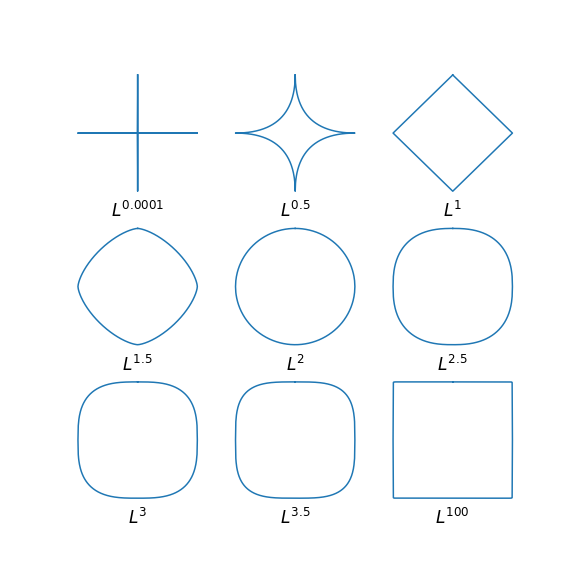
\includegraphics[width=\textwidth]{unitsets.png}
    \caption{Unit Circles: Level sets $\{\mathbf{x}: ||\mathbf{x}||_q = 1\}$ for different $L^q$ norms.}
    \label{fig:svd_eigenfaces}
\end{figure}


\subsection{$L^{1}$ Taxicab / Manhattan Norm}
\label{sec:l1norm}
\begin{equation}
||\mathbf{x}||^1 = \sum_i |x_i|
\end{equation}

In the context of regression, $L^1$ loss gives the maximum likelihood estimator under the assumption of Laplacian (double exponential) distributed errors. For a dataset $\mathbf{x}\in S$, minimizing $\argmin_{\mathbf{s}} \sum_{\mathbf{x}\in S}||\mathbf{x}-\mathbf{s}||_{1}$ gives the median.


\subsection{$L^{2}$ Euclidian Norm}
\label{sec:l2norm}
\begin{equation}
||\mathbf{x}||^2 = \sum_i |x_i|^2
\end{equation}


In the context of regression, $L^2$ loss gives the maximum likelihood estimator under the assumption of normally distributed errors. For a dataset $\mathbf{x}\in S$, minimizing $\argmin_{\mathbf{s}} \sum_{\mathbf{x}\in S}||\mathbf{x}-\mathbf{s}||_{2}$ gives the mean.

I believe that $L^2$ norm should be the only norm that preserves the distance between two points under rotations of the coordinate system.	

\subsection{$L^{\infty}$ Maximum Norm} 

\begin{equation}
||\mathbf{x}||^{\infty} = \max(x_1,x_2,...,x_n)
\end{equation}

For a dataset $\mathbf{x}\in S$, minimizing $\argmin_{\mathbf{s}} \sum_{\mathbf{x}\in S}||\mathbf{x}-\mathbf{s}||_{\infty}$ gives the average of the maximum and the minimum value of the dataset.


\subsection{$L^{-\infty}$ Minimum Norm} 

Formally, I only came across values $0<p$, but it is my opinion that $-\infty$ picks out the minimum value:

\begin{equation}
||\mathbf{x}||^{-\infty} = \min(x_1,x_2,...,x_n)
\end{equation}





\section{Operator and Matrix Norms}
\label{sec:norms}

Matrix norms are functions $||\cdot||: K^{m\times n} \rightarrow \mathbb{R}$ where $K$ is a field of real or complex numbers. They satisfy:

\begin{itemize}
\item $||\alpha A|| = |a| ||A||$ (absolutely homogenous)
\item $||A+B|| \leq ||A|| + ||B||$ (triangle inequality, subadditivity)
\item $||A||\geq 0$ (positive valued)
\item $||A||=0 \implies A_{n,m}=0$ (definiteness)
\end{itemize}

A norm is submultiplicative if it satisfies $||AB||\leq||A||||B||$, which \citeasnoun{rgeraNotes} calls a requirement of "useful matrix norms".

\subparagraph{} 
The main risk of confusion is that norms for operators and vectors are different animals. Norms for operators normally measure some relationship between input and output. Norms for vectors are normally some kind of size, length or distance metric. In as far as matrices can be thought of as both operators and multidimensional vectors, norms of either type may be applied to them. People's notation and language is all over the place. Below I've used $||\cdot||_{(\alpha)}$ to denote norms in the operator sense and $||\cdot||_{\alpha}$ in the vector sense. 

\subsection{$||\mathbf{A}||_{(\alpha)}$ Operator Norm}
\label{sec:operatornorm}
The operator norm describes the largest change in size that it may impart on any of its inputs. That means that the operator norm is defined with respect to a definition of size in both domain and codomain. I.e., for an operator $\mathbf{A}$ and a given way of measuring size $||\cdot||_{\alpha}$:

\begin{equation}
||\mathbf{A}||_{(\alpha)} = \sup\left\{\frac{||\mathbf{A}\mathbf{v}||_{\alpha}}{||\mathbf{x}||_{\alpha}}: \mathbf{v} \in V\right\}
\end{equation}

When the operator is given by a matrix $\mathbf{A}$, and the length of the vector $\mathbf{x}$ is measured using the usual euclidian 2-norm ($||\cdot||_{2}$), then the operator norm is given by the square root of the largest eigenvalue of $\mathbf{A^T A}$. In that case, the operator norm is the same as the 2-norm (cf. section \ref{sec:2norm}).

To re-emphasize, $||A||_{(q)}$ and $||A||_q$ are two different things. The former measures the change in input size, where the size of the input is measured according to the latter. That is the reason for why the 1-Norm and 2-Norms are so different from the vector norms $L_1$ and $L_2$.

Operators that preserve the length of a vector with respect to some norm $||\cdot||_{\alpha}$ satisfy $||\mathbf{A}||_{(\alpha)} = 1$ and are called isometries (cf. section \ref{sec:isometric}). 

% q-norm
\subsection{$||\mathbf{A}||_q$ $q$-Norms}
\label{sec:qnorms}

The $q$ norms for a matrix $\mathbf{A} \in \mathbb{R}^{m\times n}$ with entries $a_{i,j}$ in row $i$ and column $j$ are defined:

\begin{equation}
||\mathbf{A}||_q = \left(\sum_{i}\sum_{j} a^q_{i,j}\right)^{1/q}
\end{equation}

For $q=2$, this becomes the Frobenius norm (section \ref{sec:frobenius}). For vectors $\mathbf{v}\in\mathbb{R}^{n}$, the $q$-norm is more known as $p$-norm or $L^p$ norm (cf. section \ref{sec:lpnorms}). 


% frobenius
\subsection{$||\mathbf{A}||_F$ Frobenius Norm}
\label{sec:frobenius}
The Frobenius Norm is the sum of the squares of all entries of a matrix. Let $\mathbf{A} \in \mathbb{R}^{m\times n}$ be a matrix with entires $a_{i,j}$ in row $i$ and column $j$, then:

\begin{equation}
||\mathbf{A}||_F = \sqrt{\sum_{i}\sum_{j} a^2_{i,j}}
\end{equation}

The Frobenius norm is invariant under rotations, and $||\mathbf{A}||_F = \sqrt{\sum_i \sigma_i^2}$ where $\sigma_i$ are the singular values of $\mathbf{A}$. 

\subsection{$||\mathbf{A}||_{(1)}$ (1)-Norm}
Let $\mathbf{A}$ be a matrix with entires $a_{i,j}$ in row $i$ and column $j$, then:

\begin{equation}
||\mathbf{A}||_{(1)} = \max_{1\leq j \leq n} \sum^m_{i=1} |a_{i,j} |
\end{equation}

That is, it is the maximum of the sums of the absolute values of any of the columns of $\mathbf{A}$.

\subsection{$||\mathbf{A}||_{(\infty)}$ ($\infty$)-Norm}

Let $\mathbf{A}$ be a matrix with entires $a_{i,j}$ in row $i$ and column $j$, then:

\begin{equation}
||\mathbf{A}||_{(\infty)} = \max_{1\leq i \leq m} \sum^n_{j=1} |a_{i,j} |
\end{equation}

That is, it is the maximum of the sums of the absolute values of any of the rows of $\mathbf{A}$.

\subsection{$||\mathbf{A}||_{(2)}$ (2)-Norm}
\label{sec:2norm}

Let $\mathbf{A} \in \mathbb{R}^{m\times n}$ be a matrix with entires $a_{i,j}$ in row $i$ and column $j$, then:

\begin{equation}
||A||_{(2)} = \max_{\mathbf{x}\neq 0} \frac{||\mathbf{Ax}||_2}{||\mathbf{x}||_2}
\end{equation}

Which is the square root of the largest eigenvalue of $A^T A$. Or, equivalently, $||A||_{(2)} = \sigma_1$, where $\sigma_1$ is the largest singular value of the SVD of $\mathbf{A} = \mathbf{U\Sigma V}^T$. That means that $||A^{-1}|| = \frac{1}{\sigma_n}$, where $\sigma_n$ is the smallest singular value of the SVD of $\mathbf{A}$. 




